\section{MVC-mønsteret}\label{MVC}
Et af de standardiserede design mønstre, som bruges af mange udviklere er MVC-mønsteret - som står for \textit{Model-View-Controller}.
MVC-mønsteret har til formål, at dele systemet op i tre komponenter, nemlig \textit{Model}, \textit{View} og \textit{Controller}.
Denne segregering adskiller således ''forretnings-logik'', ''input-logik'' og ''UI-logik'', og gør herved systemet mere fleksibelt, samt fremmer muligheden for at udvikle parallelt på de forskellige komponenter.
Dette kan være nyttigt i udviklingen af systemet, men også efter udgivelsen, idet blandt andet ''UI-logik''kan blive ændret oftere end for eksempel ''forretnings-logik''.
Opdelingen hjælper også til at skabe overblik over koden, og gør det nemmere at udføre tests på systemet. \citep{MVC_Overview}

\begin{wrapfigure}{r}{0.4\textwidth}
	\vspace{-20pt}
	\begin{center}
		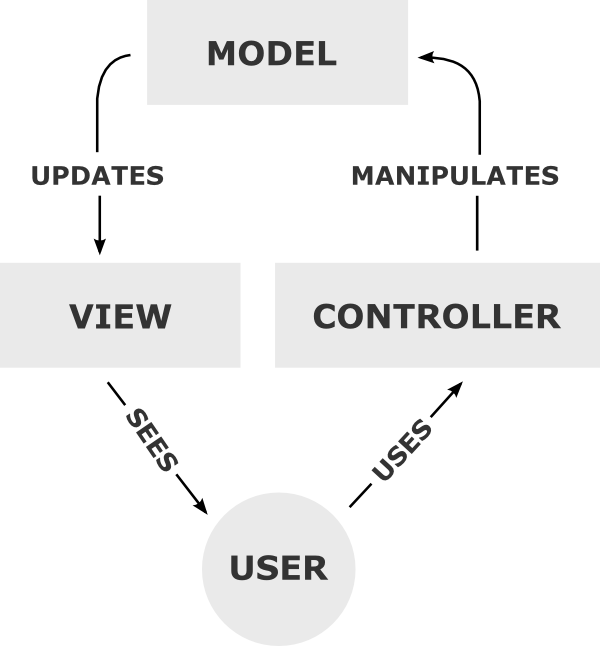
\includegraphics[width=0.38\textwidth]{images/Images/mvc.png}
	\end{center}
	\vspace{-20pt}
	\caption{MVC-mønsteret}
	\vspace{-20pt}
\end{wrapfigure}


Nedenfor beskriver vi de tre komponenter.

\textbf{Model}\\
De objekter, der udgør model-laget skal indeholde den før omtalte ''forretnings-logik'', samt alle data der skal modelleres i systemet.
Dataen, i form af objekter, gemmes oftest i en database eller fil, og er helt skjult for brugeren i den forstand, at al repræsentation af modellen foregår igennem view-delen af MVC-mønsteret.

\textbf{View}\\
Der er igennem forskellige views, at brugeren får præsenteret brugergrænsefladen - også kaldet UI(user-interface).
Derfor giver det også mening, at placere ''UI-logikken'' i denne del af MVC-mønsteret.
Typisk bliver et views indhold genereret ud fra data fra en model.
Et eksempel på dette ville være visning af en liste af objekter ud fra en model, der indeholder netop en liste.

\textbf{Controller}\\
Når det kommer til interaktionen mellem brugeren og systemet, er det controlleren der påtager sig opgaven.
Derfor er det også i de forskellige controllerere, at vi finder ''input-logikken''. Her bestemmes ud fra input fra brugeren hvilke data der skal arbejdes med i hvilken model og også hvilket view, der skal præsenteret for brugeren. Med dette kan vi også se, at viewet ikke indeholder nogenb logik og al manipulation af data altså foregår gennem controller komponenten.
